\documentclass{scrartcl}
% \usepackage{german} % including this twice is causing build fails !!
\usepackage[utf8]{inputenc}
\usepackage[german]{babel}
\usepackage{amssymb} % what does it do?
\usepackage{graphicx} % I can't do that yet
\usepackage{fancyhdr} % what does it do?
\usepackage{lastpage} % what does it do?
\setlength{\parskip}{\medskipamount} % thats reasonable
\setlength{\parindent}{0pt} % whatever that does


%%%%%%%%%%%%%%%%%%%%%%%%
% Kopf- und Fusszeilen %
%%%%%%%%%%%%%%%%%%%%%%%%
\pagestyle{fancy}
\lhead{
    \begin{tabular}{ll}
        Felix Karg \\
    \end{tabular}
}
\chead{Bioinformatics Handout}
\rhead{
    \begin{tabular}{rr}
        \today{} \\
        Page \thepage{} of \pageref{LastPage}
    \end{tabular}
}
\lfoot{}
\cfoot{}
\rfoot{}

%%%%%%%%%%%%%%%%%%%%%%%%
% Anfang des Dokuments %
%%%%%%%%%%%%%%%%%%%%%%%%
\begin{document}

\section*{A Simple Protocol for the Inference of RNA Global Pairwise Alignments}






Secondary structures are usually similiar in functionally similiar regions


\subsection*{SPS}
Is called the Sum of Pairs Score, Similiarity is: \\
1 - (edit distance / unaligned length of shorter sequence)

\subsection*{Sequence Identity}
The identity is the number of identical nucleotides divided by the shorter sequence length


\subsection*{needle}

needle is an implementation of the sequence based Needleman-Wunsch algorithm.

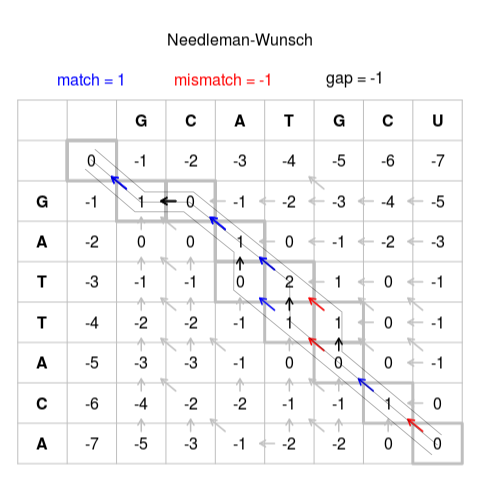
\includegraphics[width=0.7\textwidth]{proseminar/images/Needleman-Wunsch_pairwise_sequence_alignment}

\newpage


\subsection*{Sequence Alignment}

There's three categories:
\begin{itemize}
\item local
\item global 
\item glocal
\end{itemize}

Local is comparing (local) parts which are pretty similiar to begin with.

Global is just comparing two RNA strands, complete.

Glocal is roughly everything else, having restrictions (beginning/end) when aligning.


\subsection*{LocARNA}

Is a folding and aligning sequence algorithm.

First a base pair probability matrix is being created using RNAfold.

Then this is used as a guide for optimal alignment.


\subsection*{Tree-based Sequence Alignments}

\begin{itemize}
\item gardenia
\item RNA StrAT
\item RNAdistance
\item RNAforester
\end{itemize}

These are also extensively using the secondary structure.


\subsection*{Comparison}

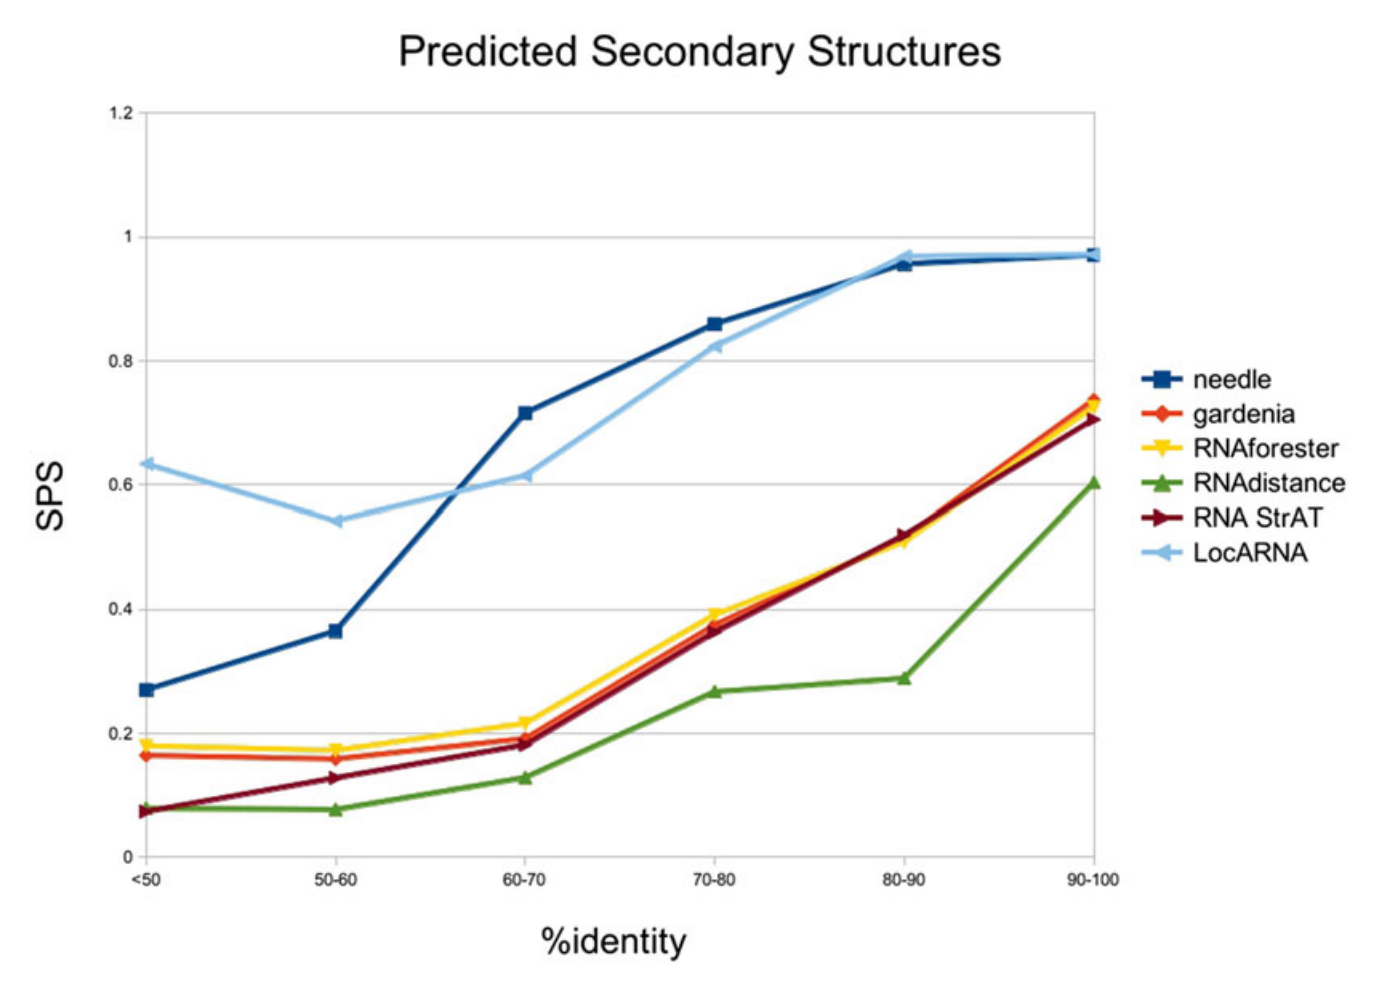
\includegraphics[width=0.9\textwidth]{proseminar/images/predicted} \\
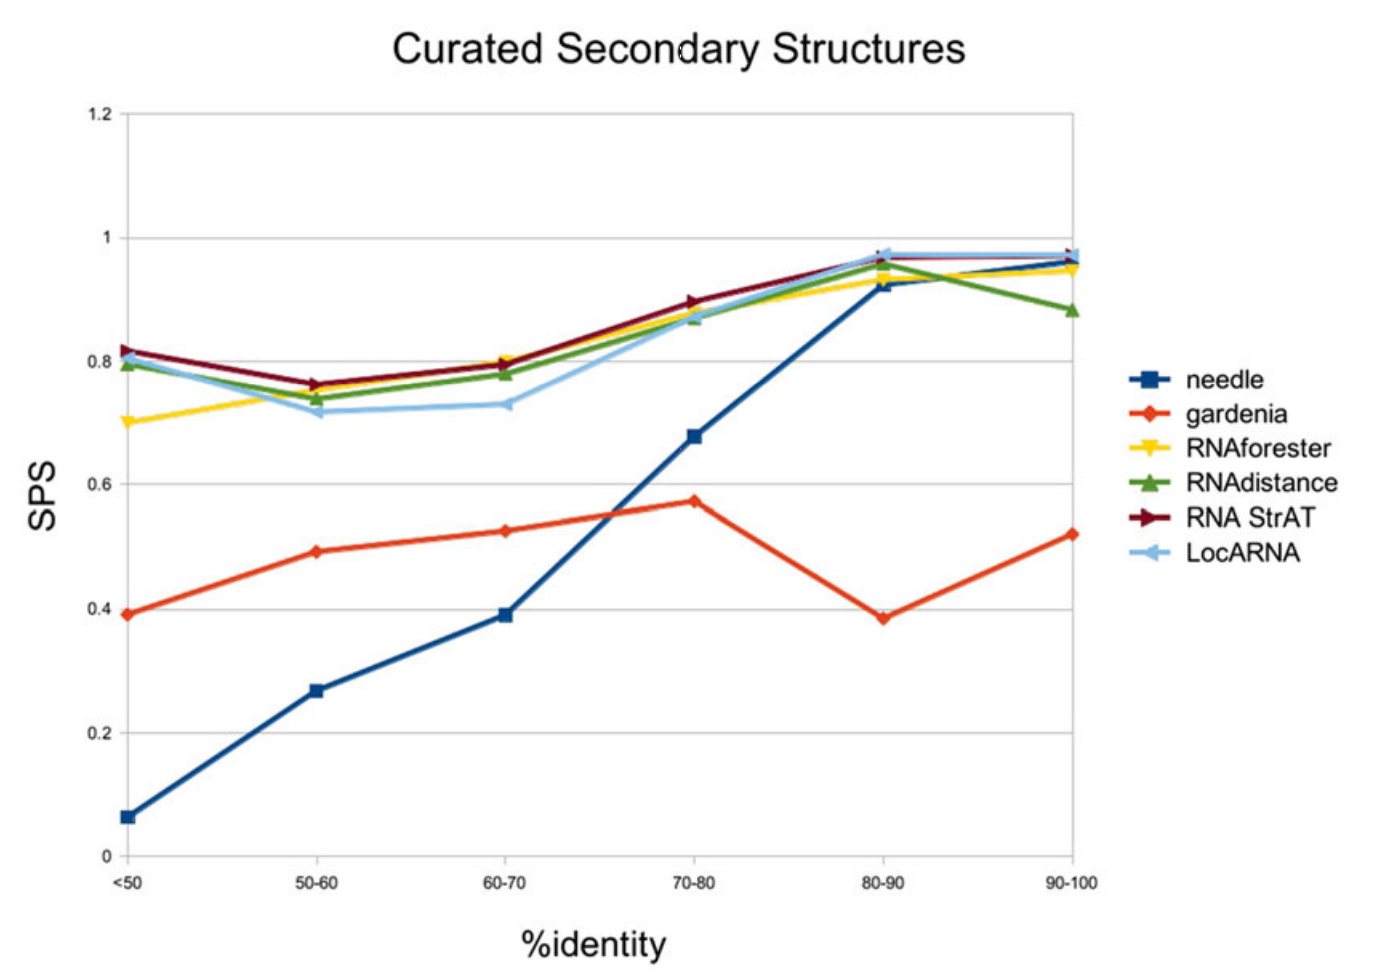
\includegraphics[width=0.9\textwidth]{proseminar/images/curated}




\end{document}


